\documentclass[12pt, a4paper, oneside]{article}
%die Pakete werden hier durch den Include-Befehl separat eingelesen

% Pakete für die Literaturverwaltung und Zitieren im APA-Stil
\usepackage[utf8]{inputenc}
\usepackage[ngerman]{babel}
\usepackage{csquotes}
\usepackage[backend=biber,style=apa]{biblatex}
\DeclareLanguageMapping{ngerman}{ngerman-apa}
\usepackage[bottom]{footmisc}

% Pakete für die Darstellung von Bildern
\usepackage{graphicx}
\usepackage{floatflt}

% Mathematik-Pakete
\usepackage{amsmath}
\usepackage{amsfonts}
\usepackage{amssymb}
\usepackage{dsfont}

% Weitere Pakete
\usepackage{microtype}
\usepackage{footnote}
\makesavenoteenv{tabular}
\usepackage{blindtext}
\usepackage{etoolbox}
\usepackage[list]{acro}
\usepackage[onehalfspacing]{setspace}
\usepackage[top=3cm, bottom=2cm, left=3cm, right=2cm]{geometry}
\usepackage{tabularx}
\usepackage{adjustbox}
\usepackage{epsfig}
\usepackage{longtable}
\usepackage{dcolumn}
\usepackage{here}
\usepackage{xcolor}
\usepackage{listings}
\usepackage{lipsum}
\usepackage{dirtree}
\usepackage{afterpage}
\usepackage[pdfborderstyle={/S/U/W 1}]{hyperref} %Nur verwenden wenn Links im Dokument farbig angezeigt werden sollen
%\usepackage[hidelinks]{hyperref} %Verwenden wenn die Links nicht farbig hervorgehoben werden sollen.
\usepackage{xurl}

% Benutzerdefinierte Befehle
\newcommand{\ricardo}[1]{\colorbox{ForestGreen}{\color{white}   \textsf{\textbf{Ricardo}}} \textcolor{ForestGreen}{#1}}

% Schriftart auf Sans-Serif ändern
\renewcommand{\familydefault}{\sfdefault}

% Hier geben Sie Ihre Bibliografiedatei an
\addbibresource{Bibliographie.bib}

\DeclareAcronym{Vgl.}{
    short = Vgl.,
    long = Vergleiche
}

\newcommand{\autor}{Dein Name}
\newcommand{\street}{Deine Straße}
\newcommand{\placeOfResidence}{Deine Wohnort}
\newcommand{\studyTitle}{Dein Studiumstitel }
\newcommand{\studyProgram}{Dein Studiumsprogramm}
\newcommand{\studyGroup}{Deine Studiengruppe}
\newcommand{\titel}{Dein Abschlussarbeitstitel}
\newcommand{\deliveryDate}{Dein Abgabedatum}
\newcommand{\prof}{Dein Prof}


% Setze die Optionen für das Abkürzungsverzeichnis
\acsetup{
    list/template = longtable,
    first-style=short
}

\graphicspath{ {./Images/} }

\lstset{language=R}
\lstset{basicstyle=\ttfamily,
    basicstyle=\small}
\lstset{literate=%
    {Ö}{{Ö}}1
    {Ä}{{Ä}}1
    {Ü}{{Ü}}1
    {ß}{{\ss}}1
    {ü}{{ü}}1
    {ä}{{ä}}1
    {ö}{{ö}}1
}

% YAML lstset
\lstdefinelanguage{YAML}{
    keywords={true,false,null,y,n},
    keywordstyle=\color{blue},
    sensitive=false,
    comment=[l]{\#},
    commentstyle=\color{gray}\ttfamily,
    stringstyle=\color{orange}\ttfamily,
    morestring=[b]',
    morestring=[b]"
}

% JSON lstset
\lstdefinelanguage{JSON}{
    keywords={true,false,null},
    keywordstyle=\color{blue},
    sensitive=false,
    comment=[l]{//},
    morecomment=[s]{/*}{*/},
    commentstyle=\color{gray}\ttfamily,
    stringstyle=\color{orange}\ttfamily,
    morestring=[b]',
    morestring=[b]"
}

% XML lstset
\lstdefinelanguage{XML}{
    basicstyle=\ttfamily\footnotesize,
    morestring=[b]",
    morestring=[s]{>}{<},
    morecomment=[s]{<?}{?>},
    morecomment=[s]{<!--}{-->},
    commentstyle=\color{gray},
    keywordstyle=\color{blue},
    stringstyle=\color{orange},
    morekeywords={xmlns,version,type,project,modelVersion,parent,groupId,artifactId,packaging,name,description,properties,java,siemens,tc,,log4j2,spring,openapi,oracle,jdbc,dependencies,dependency,groupId,exclusions,exclusion,build,configuration,finalName,xsi,schemaLocation,plugins,plugin,executions,execution,id,phase,goals,goal,defaultLibBundleDir,skinnyWars,displayName,modules,webModule,contextRoot,scope}% list your attributes here
}

\lstset{
    frame=single,
    breaklines=true,
    postbreak=\raisebox{0ex}[0ex][0ex]{\ensuremath{\color{red}\hookrightarrow\space}},
    backgroundcolor=\color{white},
    basicstyle=\ttfamily\small,
    numbers=left,
    numberstyle=\tiny\color{gray},
    showstringspaces=false,
    tabsize=2,
    rulecolor=\color{black!30},
    captionpos=b
}


\title{\textbf{Bachelor Thesis}}
\author{Mauritz Langer}

\setlength{\parindent}{0cm} %keine Einrückung
\linespread{1.5}

\newcounter{SeitenzahlSpeicher}
\begin{document}

    \setcounter{tocdepth}{4} % Include paragraphs in table of contents
    \setcounter{secnumdepth}{4} % Number paragraphs

    \thispagestyle{plain}

%\newcommand\tab[1][1cm]{\hspace*{#1}}

\begin{titlepage}

    
\includegraphics[scale=0.5]{Images/ihk-logo}
    \hfill
    
\includegraphics[scale=1]{Images/w-hs-logo}

    \vspace*{4em}


    \begin{center}
        \normalsize

        \Huge{\textbf{Abschlussarbeit}}\\[1em]

        \Large{\textbf{\titel}}\\[6em]


    \end{center}
    \large

    \begin{table}[b!]
        \large
        \setlength{\tabcolsep}{30pt}
        \begin{tabular}{@{\extracolsep{2cm}}ll@{\extracolsep{1cm}}}
            vorgelegt von:     & \textbf{\autor}     \\
            & \street            \\
            & \placeOfResidence            \\
            \\
            Studiengang:       & \studyTitle \\
            & \studyProgram        \\
            & \studyGroup      \\
            \\
            Themensteller/ & \prof               \\
            Betreuer:& \\
            \\
            Abgabedatum:       & \deliveryDate        \\
        \end{tabular}
    \end{table}

\end{titlepage}
\clearpage


    \begin{spacing}{1}
        \pagenumbering{Roman}
        \setcounter{page}{1}
        \tableofcontents
    \end{spacing}

    \newpage
    \begin{spacing}{1}
        \section*{Abkürzungsverzeichnis}
        \addcontentsline{toc}{section}{Abkürzungsverzeichnis}
        \printacronyms[heading=none]
    \end{spacing}

    \newpage
    \begin{spacing}{1}
        \section*{Abbildungsverzeichnis}
        \addcontentsline{toc}{section}{Abbildungsverzeichnis}
        \renewcommand{\listfigurename}{}
        \listoffigures
    \end{spacing}

    \newpage
    \begin{spacing}{1}
        \section*{Tabellenverzeichnis}
        \addcontentsline{toc}{section}{Tabellenverzeichnis}
        \renewcommand{\listtablename}{}
        \listoftables
    \end{spacing}

    \newpage
    \clearpage
    \setcounter{SeitenzahlSpeicher}{\value{page}}
    \pagenumbering{arabic}
    \newpage
    \pagenumbering{arabic}

    \section{Einleitung}

\subsection{Motivation}\label{subsec:motivation}

Lorem ipsum dolor sit amet, consectetur adipiscing elit. Vestibulum pretium quam eget venenatis consectetur.
Donec mollis nisi nulla, pellentesque semper est mollis ac.
Etiam tincidunt pellentesque risus, id ornare purus imperdiet at.
Integer pulvinar iaculis condimentum.
Duis vel libero odio.
Nullam dignissim vel sem vel vestibulum.
Interdum et malesuada fames ac ante ipsum primis in faucibus.
Mauris quis augue at velit rhoncus elementum at ac purus.\\
Ut augue sem, sagittis aliquam ante at, efficitur faucibus enim.
Phasellus accumsan, nisi non volutpat elementum, libero sapien sagittis velit, ut euismod leo ipsum non sem.
Phasellus ultrices tempus blandit.
Nunc bibendum nibh et dolor lobortis ullamcorper.
Quisque congue in urna id pretium.
Duis volutpat ultrices felis sagittis elementum.
Nullam aliquet ante nec cursus fermentum.
Praesent id semper nisl.
Nunc sagittis porttitor mi sit amet rutrum.
Ut porta ligula et augue fringilla interdum a et eros.
Suspendisse urna eros, aliquet ut ante tempus, interdum faucibus nisi.
Donec quis massa ornare, viverra risus id, semper lorem.
Praesent massa tortor, ultrices id nulla et, placerat rhoncus sem.
Cras posuere ipsum quis ex dictum, a aliquet ligula efficitur.
Maecenas eu fermentum odio.
Nulla eget arcu in lorem dapibus rhoncus eget nec est.

\subsection{Zielsetzung}

Proin ornare elit leo, sit amet molestie orci facilisis a.
Sed eget luctus velit.
Duis placerat nisl felis, et scelerisque dui finibus id.
Nam ornare blandit metus, ac dapibus mauris blandit non.
Nam ut felis sagittis, mattis ex a, ornare lorem.
Aliquam id leo tempus, feugiat elit nec, sagittis lorem.
Etiam porta blandit quam quis suscipit.\\
Cras eu ipsum at massa viverra tincidunt at sit amet sapien.
Pellentesque quis eleifend erat, vitae accumsan risus.
Morbi ultricies turpis quis rutrum posuere.
Etiam ante risus, placerat eu bibendum sed, mollis sit amet nunc.
Aenean semper placerat finibus.
Pellentesque tincidunt sed sem sed dictum.
Aliquam fermentum volutpat leo non laoreet.
Proin aliquet accumsan eros vel efficitur.
Quisque non risus luctus, elementum ante non, laoreet risus.
Nam vulputate ligula commodo, maximus lorem ac, maximus risus.
Nunc pellentesque rhoncus dui. Duis non velit turpis.

\subsection{Aufbau}

Aliquam eget tortor augue.
Praesent bibendum blandit felis, pretium mattis leo pharetra at.
Duis rutrum dui a est pharetra tempor.
Suspendisse potenti. Suspendisse potenti.
Vivamus ac lorem eu metus vehicula tempus et et urna.
In risus leo, suscipit quis quam sit amet, cursus sodales erat.
Donec pretium vitae lacus sit amet tristique.\\
Duis aliquet, ex vitae ullamcorper vestibulum, justo eros consequat libero, sit amet pharetra libero ligula non arcu.
Integer enim urna, viverra non semper pretium, cursus vitae lectus.
Nam ac gravida sapien, eget malesuada nisl.
Nunc dapibus finibus sem.
Donec viverra lacus non metus auctor, ut egestas dui viverra.
Praesent mollis ipsum vel iaculis tristique.
Proin malesuada non tortor sollicitudin elementum.
Nulla vitae neque eu nisi ultrices tincidunt.
Donec porta, enim sit amet egestas scelerisque, ante urna consectetur massa, vel vestibulum massa tellus non metus.

\section{Verweise}\label{sec:grundlagen}

\subsection{Verweise auf Kapitel, Bilder und Tabellen}

Verweise auf Kapitel, Bilder oder Tabellen werden in LaTeX mithilfe von Labels und Referenzen durchgeführt.
Beispielweise muss bei dem zu referenzierenden Objekt ein Label angelegt werden.
Ein Beispiel für so ein Label finden Sie im ersten Kapitel.
Nun kann mittels einer Referenz auf dieses Label verwiesen werden: Kapitel~\ref{subsec:motivation}





\subsection{Quellenverweise}

Quellenverweise werden in dieser Vorlage mit dem folgenden Befehl verfasst:
\footnote{\ac{Vgl.}~\textcite{qualls_protected_2023}, \url{https://docs.gitlab.com/ee/user/project/protected_branches.html}.}\\
Zuerst wird eine neue Fußnote angelegt.
Anschließend folgt eine Definition eines Akronyms, welches zu dem Vgl.-Akronym führt.
Nun folgt der eigentliche Verweis auf die Quelle.
Diese Quelle muss vorher in der Bibilographie.bib-Datei hinterlegt worden sein.
Je nach den Anforderungen kann jetzt noch eine URL hinterlegt werden, die schnell auf eine Internet-Quelle verweist.


\section{Verzeichnisse}\label{sec:charakterisierung-der-ausgangssituation}

\subsection{Inhaltsverzeichnis}

Das Inhaltsverzeichnis wird automatisch von LaTeX erstellt.
Mithilfe der section und subsection Befehle werden neue Kapitel und Unterkapitel definiert.

\subsection{Abkürzungsverzeichnis}

Das Abkürzungsverzeichnis wird genau wie das Inhaltsverzeichnis automatisch aus den in der Acronyms.tex Datei angegebenen Akronymen erstellt.



\subsection{Abbildungsverzeichnis}

Das Abbildungsverzeichnis wird automatisch aus allen definierten Abbildungen erstellt.

\subsection{Tabellenverzeichnis}\label{sec:}

Das Tabellenverzeichnis wird automatisch aus allen definierten Tabellen erstellt.


\section{Figuren und Tabellen}\label{sec:erstellung-eines-soll-konzeptes}

\subsection{Abbildungen}

Im folgenden finden Sie die Definition für die Einbindung einer Abbildung.

\begin{figure}[h!]
  \centering
  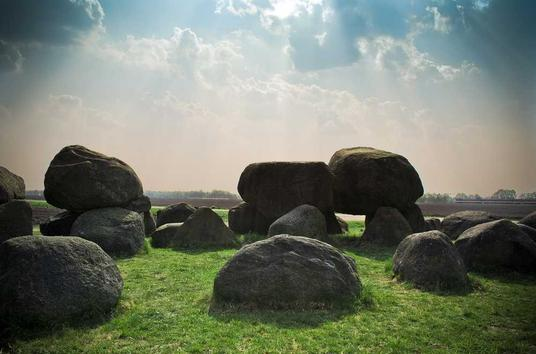
\includegraphics[scale=0.2]{Images/example}
  \caption[Example Image.]{Example Image. Quelle: eigene Darstellung.}
  \label{fig:example_image}
\end{figure}

\subsection{Tabellen}

Im folgenden finden Sie ein Beispiel für die Definition einer Tabelle.

\begin{table}[h!]
  \centering
  \setlength{\extrarowheight}{5pt}
  \begin{tabular}{|c|c|c|c|}
    \hline
    \textbf{Commit-Nachricht} & \textbf{Alte Version} & \textbf{Pre-Release} & \textbf{Release} \\
    \hline
    fix(\ldots): \ldots & 1.0.0 & 1.0.1-stage.1 & 1.0.1\\
    \hline
    feat(\ldots): \ldots & 1.0.0 & 1.1.0-stage.1 & 1.1.0\\
    \hline
    perf(\ldots): \ldots & 1.0.0 & 2.0.0-stage.1 & 2.0.0\\
    \hline
  \end{tabular}
  \caption[Commit-Nachrichten zur Erhöhung der Versionsnummer.]{Commit-Nachrichten zur Erhöhung der Versionsnummer. Quelle: eigene Darstellung.}
  \label{tab:semantic-release}
\end{table}

\subsection{Code}

Im folgenden finden Sie ein Beispiel für die Einbindung von Quellcode in die Arbeit.
Allerdings muss dazu zuerst die Sprache definiert werden.
Die Definition finden Sie in der main.tex-Datei.

\begin{spacing}{1}
  \lstinputlisting[label={lst:example}, language=XML]{Scripts/example.xml}
\end{spacing}

\subsection{Baumstrukturen}\label{subsec:prozessorientierte-auswahl-der-werkzeuge}

Im folgenden ist die Einbindung einer Baumstruktur zu finden.

\begin{figure}[h!]
  \dirtree{%
    .1 /.
    .2 test.
    .3 example.
    .4 lorem.
    .5 ipsum.
    .6 dolor.
    .7 sit.
    .5 amet.
    .6 consectetur.
    .7 elit.
  }
  \caption[Dateipfadstruktur.]{Dateipfadstruktur. Quelle: eigene Darstellung.}
  \label{fig:dateipadstruktur}
\end{figure}




    \clearpage
    \pagenumbering{Roman}
    \setcounter{page}{\theSeitenzahlSpeicher}


    \section{Literaturverzeichnis}
    \renewcommand{\refname}{}
    \printbibliography

    \newpage


    \appendix %Anhang
    \pagenumbering{arabic}


    \section{Anhang}

\subsection{Graphiken}

\begin{figure}[h!]
    \centering
    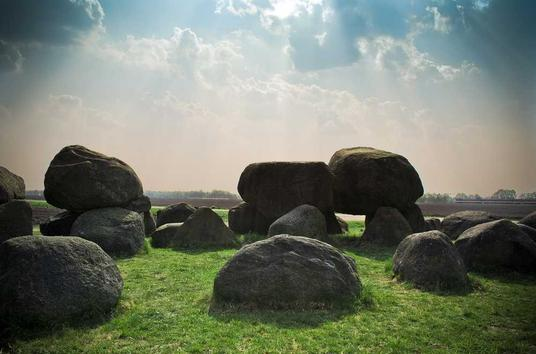
\includegraphics[scale=0.9]{Images/example}
\end{figure}

\subsection{Code-Dateien}

\begin{spacing}{1}
    \lstinputlisting[label={lst:.gitlab-ci.yml}, language=YAML]{Scripts/example.yml}
\end{spacing}

\newpage

\section{Ehrenwörtliche Erklährung}
„Ich versichere, dass ich diese Bachelorarbeit selbständig angefertigt, alle Hilfen und Hilfsmittel angegeben und alle wörtlich oder dem Sinne nach aus Veröffentlichungen oder anderen Quellen, auch dem Internet entnommenen Inhalte, kenntlich gemacht habe.“
\\$~~$\\
\\$~~$\\
\vspace{50pt}
\noindent\rule{5cm}{.4pt}\hfill\rule{5cm}{.4pt}\par
\noindent Ort, Datum \hfill Unterschrift


\clearpage


\end{document}
